% Dies ist Teil der Vorlesung Physik auf dem Computer, SS 2012,
% Axel Arnold, Universitaet Stuttgart.
% 
% Dieses Werk ist unter einer Creative Commons-Lizenz vom Typ
% Namensnennung-Weitergabe unter gleichen Bedingungen 3.0 Deutschland
% zugänglich. Um eine Kopie dieser Lizenz einzusehen, konsultieren Sie
% http://creativecommons.org/licenses/by-sa/3.0/de/ oder wenden Sie sich
% schriftlich an Creative Commons, 444 Castro Street, Suite 900, Mountain
% View, California, 94041, USA.

\chapter{Differentialgleichungen}
\index{Differentialgleichung}

Fast alle physikalischen Probleme können durch Differentialgleichungen
(DGLs) beschrieben werden. Auch das einleitende Problem des
Fadenpendels ist wurde ja durch die Differentialgleichung
\begin{equation}
  \ddot\alpha = -\frac{g}{l}\sin(\alpha)
\end{equation}
beschrieben. Die analytische Lösung dieser und der meisten
Differentialgleichungen ist schwierig oder unmöglich, und daher sind
numerische Verfahren zum Lösen von DGLs wichtige Hilfsmittel, um
Modelle mit komplexen DGLs untersuchen zu können.

Im folgenden werden wir numerische Löser für verschiedene Klassen von
Differentialgleichungen kennenlernen. Für gewöhnliche
Differentialgleichungen mit skalarer Variable sind das die
Runge-Kutta-Verfahren, sowie das bereits in der Einleitung
besprochene, sehr gebräuchliche Velocity-Verlet-Verfahren.

Schwieriger ist die Lösung partieller Differentialgleichungen, die
mehrdimensionale Variablen und deren Ableitungen enthalten.  Diese
spielen besonders in der Physik eine wichtige Rolle, weil sie bei bei
zeit- und ortsabhängigen Prozessen quasi automatisch auftreten. Hier
lernen wir einige Bespiele kennen und wie diese mit Hilfe finiter
Differenzen oder Fouriertransformationen numerisch gelöst werden
können.

\section{Gewöhnliche Differentialgleichungen}
\index{Differentialgleichung>gewöhnliche}
\index{Differentialgleichung>explizite}

Wir betrachten Differentialgleichungen der Form
\begin{equation}
  \label{eq:explicitode}
  f^{(m)}(t) = F(t, f(t), \dot f(t), \ldots, f^{(m-1)}(t))
\end{equation}
mit $f:\RR\to\RR^n$. Diese heißen gewöhnlich, da sie nur von einer
Variablen, $t$ abhängen. Wie der Name $t$ schon vermuten lässt, wird
diese Variable meist mit der Zeit assoziert. Die spezielle Form
\eqref{eq:explicitode} wird auch \emph{explizite} gewöhnliche
Differentialgleichung $m$-ter Ordnung genannt, da wir voraussetzen,
dass sich die Gleichung global nach $f^{(m)}(t)$ auflösen lässt, und
$m$ Ableitungen involviert sind. \emph{Implizite} Gleichungen der Form
$F(t, f(t), \dot f(t), \ldots, f^{(m-1)}(t),f^{(m)}(t)) = 0$ sind
numerisch sehr viel schwieriger zu lösen, tauchen aber in der Physik
auch seltener auf, und werden daher hier nicht weiter besprochen.

Für die numerische Lösung beschränken wir uns weiter auf gewöhnliche
Differentialgleichungen erster Ordnung, also von der Form
\begin{equation}
  \label{eq:1storderode}
  \dot f(t) = F(t, f(t)),\quad f(0)\;\text{gegeben}.
\end{equation}
Dies ist tatsächlich keine Einschränkung, da sich jede explizite
Differentialgleichung $m$-ter Ordnung in eine höherdimensionale
Gleichung erster Ordnung transformieren lässt:
\begin{equation}
  \frac{d}{dt}\begin{pmatrix}
    f(t)\\
    \dot f(t)\\
    \vdots\\
    f^{(m-1)}(t)
  \end{pmatrix}
  =
  \begin{pmatrix}
    \dot f(t)\\
    \ddot f(t)\\
    \vdots\\
    f^{(m)}(t) = F(t, f(t), \dot f(t), \ldots, f^{(m-1)}(t))
  \end{pmatrix}
\end{equation}

Die Differentialgleichung des einleitenden Beispiels
\begin{equation}
  \label{eq:fadenpendel2}
  \ddot \alpha(t) = -\frac{g}{l}\sin(\alpha(t)),
\end{equation}
wird so zum Beispiel zu
\begin{equation}
  \frac{d}{dt}\begin{pmatrix}
    \alpha(t)\\
    \dot \alpha(t)
  \end{pmatrix}
  =
  \begin{pmatrix}
    \dot \alpha(t)\\
    -\frac{g}{l}\sin(\alpha(t)),
  \end{pmatrix}.
\end{equation}  
Der Startwert ist dann $(\alpha(0), \dot \alpha(0))$, also
Anfangsposition und -geschwindigkeit.

\subsection{\keyword{Runge-Kutta-Verfahren}}

Wir betrachten nun das allgemeine Problem~\eqref{eq:1storderode}, also
\begin{equation*}
  \dot f(t) = F[t, f(t)],\quad f(0)\;\text{gegeben}.
\end{equation*}
Wir suchen eine diskretisierte Näherung $y_n \approx f(t_n)$ mit
äquidistanten Zeitpunkten $t_n=n h$, $n=0,1,\ldots$, also Schrittweite
$h$. Es gilt
\begin{equation}
  f(t_{n+1}) = f(t_n+h) = f(t_n) + \int_{t_n}^{t_n+h} \dot f(t)\,dt
  =  f(t_n) + \int_{t_n}^{t_n+h} F[t, f(t)]\,dt.
\end{equation}
Da $y_0 = f(0)$ gegeben ist, liegt es nahe, $y_1 \approx f(h)$ durch
numerische Integration zu bestimmen, dann $y_2 \approx f(2h)$ durch
numerische Integration aus $y_1$ und so weiter. Das Problem dabei ist,
dass der Integrand $F[t, f(t)]$ die zu findende Funktion $f$
enthält. Um also $f(t)$ an Stellen $t\in [t_n, t_n + h]$ annähern zu
können, müssen wir die Zwischenwerte von $f$ wiederum durch
Integration gewinnen. Dies führt zur allgemeinen Form eines
$s$-stufigen Runge-Kutta-Verfahrens
\begin{equation}
  y_{n+1} = y_n + h\sum_{j=1}^s b_j k_j
\end{equation}
mit
\begin{equation}
  \label{eq:rkkj}
  k_j = F(t + h c_j, y_n + h \sum_{k=1}^s a_{jk} k_k)
\end{equation}
und Verfahrenskonstanten $b,c\in\RR^s$ und
$A=(a_{jk})\in\RR^{s,s}$. Diese Konstanten sind dabei nicht nur nicht
von $F$ abhängig, sondern auch von der Schrittweite $h$. Ein
Runge-Kutta-Schema kann daher durch Verkleinern der Schrittweite im
Prinzip beliebig genau gemacht werden.  Die $k_j$ sind Näherungen für
$F[t + h c_j, f(t_n + h c_j)]$ und erscheinen auf beiden Seiten
von~\eqref{eq:rkkj}.  Ist $F(t,y)$ eine nichtlineare Funktion, ist
eine solche implizite Gleichung nur aufwändig zu lösen.

\index{Runge-Kutta-Verfahren>explizite}%
Daher werden meist \emph{explizite} Runge-Kutta-Verfahren verwendet,
bei denen $A$ eine linke untere Dreiecksmatrix mit Nulldiagonale ist,
also $a_{jk} = 0$ für $k\ge j$. Dann werden zur Berechnung von $k_j$
nur $k_k$, $k=1(1)j-1$ benötigt, die bereits berechnet sind. Eine
Implementierung eines Runge-Kutta-Verfahrens ähnelt dann sehr dem
Gauß-Seidel-Verfahren, dass ebenfalls die Zeilen der zu lösenden
Matrix sequentiell abarbeitet.

Das man trotzdem auch implizite Verfahren, also mit allgemeiner
Matrix, in Betracht zieht, hängt damit zusammen, dass diese stabiler
sind, und auch sogenannte steife DGLs lösen können. Ist $A$ linke
untere Dreiecksmatrix, aber die Diagonale nicht Null, spricht man von
DIRKs, diagonal-impliziten Runge-Kutta-Verfahren. Diese lassen sich
noch mit verhältnismäßig begrenztem Aufwand lösen, da pro $k_j$
lediglich eine eindimensionale Gleichung gelöst werden muss.

Der Fehler von Runge-Kutta-Verfahren wird üblicherweise durch die
Konvergenz- und Konsistenzordnung beschrieben. Die Konvergenzordnung
$p$ besagt, dass die Näherung gleichmäßig gegen $f(t_n)$ konvergiert, also
$\max \norm{y_n - f(t_n)} = \O(h^p)$. Die Konvergenz ist
meist schwer zu beweisen, einfacher ist die Konsistenzordnung $p$, die
nur fordert, dass $\norm{y_{n+1} - f(t_{n+1})} = \O(h^p)$, falls
$y_n=f(t_n)$. Konsistenz besagt also lediglich, dass ein Schritt
prinzipiell konvergiert. Ist die Funktion $F$ Lipschitz-stetig, also
etwa genügend glatt, dann gilt allerdings Konsistenzordnung =
Konvergenzordnung.

\index{Butcher-Tableau}%
Im folgenden werden einige der gebräuchlicheren Runge-Kutta-Verfahren
angegeben. Dabei hat sich das \emph{Butcher-Tableau}
\begin{center}
  \renewcommand{\arraystretch}{1.3}
  \begin{tabular}{r|l}
    c & A \\\hline
    & $b^T$
  \end{tabular}
\end{center}
als kurze Darstellung etabliert. Die $j$-te Zeile gibt an, zu welchen
Zeitpunkt $t_n + hc_j$ die Näherung $k_j$ berechnet wird, $a_{jk}$
sind die zu den benutzten Elementen $k_k$ gehörigen Gewichte der
numerischen Integration, und $b_j$ sind die Gewichte der
Näherungen $k_j$ in der Integration zu $y_{n+1}$.

Die Konstanten ergeben sich aus den benutzten
Quadraturformeln. Allerdings gibt es neben der Bedingung, dass die
Formeln möglichst explizit sein sollten, noch weitere
Stabilitätsbedingungen, die hier aber nicht beschrieben werden
können. Daher kann man nicht einfach beliebige Quadraturformeln
kombinieren, sondern sollte bei den im folgenden beschriebenen,
gebräuchlichen Formeln bleiben.

\subsubsection{Explizites Eulerverfahren}
\index{Eulerverfahren>explizites}

\begin{center}
  \renewcommand{\arraystretch}{1.3}
  \begin{tabular}{r|l}
    0 & \\\hline
    & 1
  \end{tabular}
\end{center}

Das Butcher-Tableau besagt nichts anders, als dass
\begin{equation}
  y_{n+1} = y_n + h F(t_n, y_n) \approx f(t_n) + h f'(t_n).
\end{equation}
Es handelt sich als um die direkte Integration per Rechteckregel, und
damit um ein Verfahren der Ordnung 1, d.h.\ der globale Fehler
$\O(h)$. Diese Verfahren entspricht der einfachen
Integration~\eqref{eq:simple} im einleitenden Beispiel. Das explizite
Eulerverfahren ist nicht sehr genau und nur für global
Lipschitz-stetige $F$ stabil. Daher sollte man es bei praktischen
Anwendungen im allgemeinen vermeiden.

\subsubsection{Implizites Eulerverfahren}
\index{Eulerverfahren>implizites}

\begin{center}
  \renewcommand{\arraystretch}{1.3}
  \begin{tabular}{r|l}
    1 & 1\\\hline
    & 1
  \end{tabular}
\end{center}

Wie der Name schon sagt, ist dies ein implizites Verfahren, genauer,
ein DIRK, bei dem in jedem Schritt die Gleichung
\begin{equation}
  k_1 = F(t_{n+1}, y_n + h k_1)
\end{equation}
gelöst werden muss. Dann ist die neue Näherung $y_{n+1} = y_n + h
k_1$. Durch Einsetzen ergibt sich 
\begin{equation}
  y_{n+1} = y_n + h F(t_{n+1}, y_{n+1}),
\end{equation}
das implizite Eulerverfahren ist also ebenfalls eine Rechteckregel,
aber mit dem neu zu bestimmenden Punkt $y_{n+1}$ als Aufpunkt. Die
Ordnung dieses Verfahrens ist ebenfalls 1. Anders als das explizite
Eulerverfahren ist das implizite Eulerverfahren ziemlich stabil, auch
wenn $F$ nicht Lipschitz-stetig ist. Der Nachteil ist, dass in jedem
Schritt eine nichtlineare Gleichung gelöst werden muss, was das
Verfahren recht aufwändig macht.

\subsubsection{Das Runge-Kutta-Verfahren}
\index{Runge-Kutta-Verfahren>4. Ordnung}

\begin{center}
  \renewcommand{\arraystretch}{1.3}
  \begin{tabular}{r|llll}
    0 & \\
    $\nicefrac{1}{2}$ & $\nicefrac{1}{2}$ \\
    $\nicefrac{1}{2}$ & 0 & $\nicefrac{1}{2}$ \\
    1 & 0 & 0 & 1 \\
    \hline
    & $\nicefrac{1}{6}$ &  $\nicefrac{1}{3}$ & 
    $\nicefrac{1}{3}$ &  $\nicefrac{1}{6}$
  \end{tabular}
\end{center}

Dies ist das erste Runge-Kutta-Verfahren, das zuerst 1901 von Kutta
beschrieben wurde. Wird von dem Runge-Kutta-Verfahren gesprochen, ist
daher dieses Verfahren gemeint. Bei genügend glattem $f$ hat es
Konvergenzordnung 4, ist also deutlich besser als die Eulerverfahren.

Wie können wir das Tableau verstehen?  Wir setzen
$\tau=\nicefrac{h}{2}$. Die zweite und dritte Zeile bestimmen zwei
Näherungen für $F[t_n+\tau, f(t_n+\tau)]$, zunächst mit Hilfe der
linken ($k_2$), und dann der rechten Ableitung ($k_3$). $k_4$ ist dann
eine Näherung für $F[t_n+h, f(t_n+h)]$. Diese Näherungen werden in die
Simpsonregel eingebracht, wobei $k_2$ und $k_3$ mit gleichen Gewichten
eingehen.

\subsection{Beispiel: Lotka-Volterra-Gleichungen}
\index{Lotka-Volterra-Gleichungen}

\begin{figure}
  \centering
  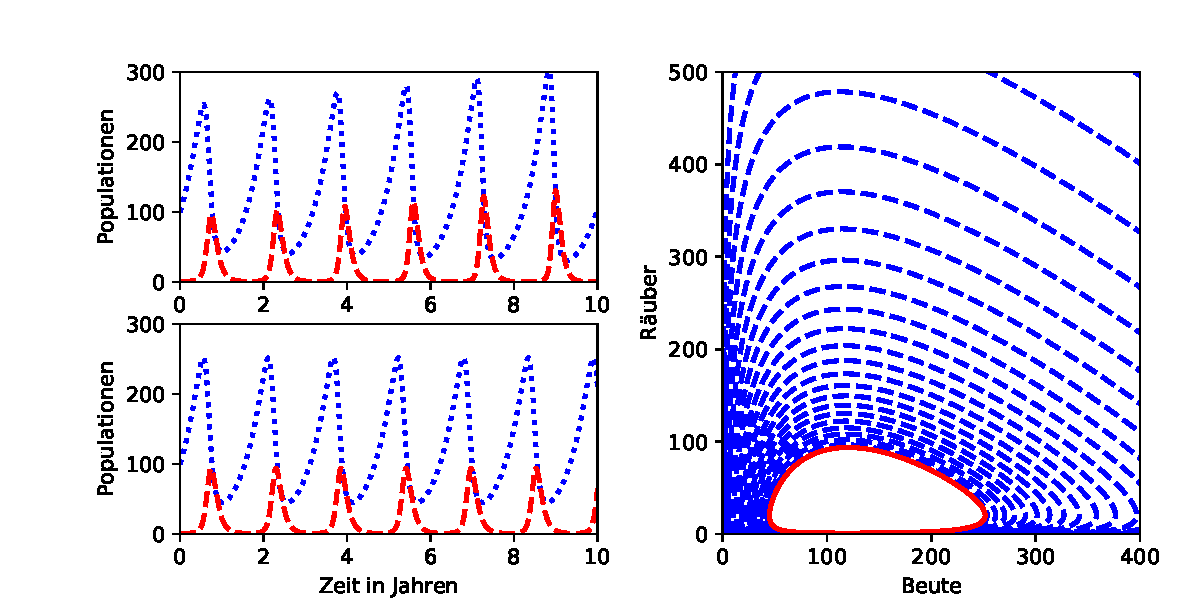
\includegraphics[width=\textwidth]{plots/lotka-volterra}
  \caption{Lösungen der Lotka-Volterra-Gleichungen mit dem einfachen
    Eulerverfahren (oben links) und dem Runge-Kutta-Verfahren (unten
    links). Blau gepunktet ist die Beutepopulation, rot gestrichelt
    die Räuberpopulation. Rechts das Räuber-Beute-Diagramm für das
    Eulerverfahren (blau gestrichelt) und das Runge-Kutta-Verfahren
    (rot durchgezogen). Während das Verfahren vierter Ordnung die
    erwartete periodische Trajektorie ergibt, wächst mit dem
    Eulerverfahren die Spitzenpopulation immer weiter. Dies zeigt die
    Instabilität des Eulerverfahrens.}
  \label{fig:lotka}
\end{figure}

Die Lotka-Volterra-Gleichungen sind nach A.~J.~Lotka und V.~Volterra
benannt, die diese 1925 als einfaches Modell für die
Populationsdynamik eines Räuber-Beute-Systems angegeben hatten, also,
wie sich die Anzahlen von Räubern und Beute im zeitlichen Verlauf
ändern.

Die Lotka-Volterra-Gleichungen sind zwei gekoppelte
Differentialgleichungen für die Populationen $N_R$ der Räuber und
$N_B$ der Beutetiere (zum Beispiel Hai und Fische, Wölfe und Hasen,
...):
\begin{equation}
  \label{eq:lotka-volterra}
  \frac{d}{dt}
  \begin{pmatrix}
    N_B\\
    N_R
  \end{pmatrix}
  = F(N_B, N_R) = 
  \begin{pmatrix}
    A N_B  - B N_BN_R\\
    -C N_R  D N_BN_R
  \end{pmatrix}.
\end{equation}
Dabei gibt $A$ die Vermehrungsrate der Beutetiere an und $B$ die Rate,
mit der ein Räuber ein Beutetier auffrisst. $C$ gibt die Sterberate
der Räuber an und $D$ die Rate, mit der sich ein Räuber vermehrt, wenn
es ein Beutetier gefangen hat. Die Räuber müssen also Beutetiere
fangen, um sich zu vermehren, während die Beutetier sich von selber
vermehren. Dieses sehr einfache Modell kennt also keine begrenzten
Resourcen, es gibt aber entsprechende Erweiterungen. Ebenso kann es
mehrstufige Systeme geben.

Im folgenden betrachten wir ein solches System aus Hasen und
Wölfen. Es sei $A=2$ Hasen pro Jahr, d.h.\ ein Hasenpaar hat vier
Nachkommen im Jahr, und $B=0,1$, ein Wolf fängt also im Schnitt alle
10 Jahre einen bestimmten Hasen. Die tatsächliche Fangrate hängt von
der Menge der Wölfe und Hasen ab. Gibt es viele Wölfe, wird es für die
Hasen eng...

Die Wölfe hingegen sind recht hungrig, wir setzen daher $C=12$. Ein
Wolf stirbt also in etwa einem Monat, wenn er keinen Hasen
fängt. Umgekehrt reicht ein Hase kaum, um sich zu vermehren, daher
setzen wir $D=0,1$, so dass etwa 10 Hasen zur erfolgreichen Vermehrung
gefressen werden müssen.

Nachdem wir nun die Raten festgelegt haben, können wir zum Beispiel
das klassische Runge-Kutta-Verfahren benutzen, um
\eqref{eq:lotka-volterra} zu lösen. Dazu müssen wir noch einen
Startwert festlegen, zum Beispiel hundert Hasen und einen Wolf, und
eine Schrittweite, die wir auf einen Tag, also $1/365$-tel,
setzen. Abbildung~\ref{fig:lotka} zeigt die resultierenden
Populationen, einmal als Funktion der Zeit und einmal als
Räuber-Beute-Diagramm.

Charakteristisch für die Lotka-Volterra-Gleichungen ist ein
periodisches Verhalten, wie man relativ leicht analytisch zeigen
kann. Dabei gibt es lediglich zwei Gleichgewichtszustände, den man
leicht bestimmen kann:
\begin{equation}
  0 \stackrel{!}{=}
  \begin{pmatrix}
    N_B (A - B N_R)\\
    N_R (-C + D N_B)
  \end{pmatrix}
  \implies N_B=N_R=0\;
  \text{oder}\;N_B=\frac{C}{D}\;\text{und}\;N_R=\frac{A}{B}.
\end{equation}
In unserem Fall wären die Populationen also bei $N_B=120$ und $N_R=20$
stabil. Unser davon leicht abweichender Startwert sollte zu einer
Trajektorie führen, die um diesen Fixpunkt periodisch kreist. Dies ist
auch tatsächlich der Fall, wenn das Runge-Kutta-Verfahren, das vierte
Ordnung hat, benutzt wird. Beim Eulerverfahren hingegen nehmen beide
Populationen mit der Zeit zu. Selbst wenn der Zeitschritt um einen
Faktor 10 gesenkt wird, driften die Populationen während der gezeigten
10 Jahre um etwa 10 Individuen. Dies zeigt eindrücklich die
Instabilität des Eulerverfahrens.

\subsection{Velocity-Verlet-Verfahren}
\index{Velocity-Verlet-Verfahren}

In der Einleitung hatten wir bereits besprochen, dass die
Fadenpendelgleichung~\eqref{eq:fadenpendel2} mit Hilfe des
Velocity-Verlet-Verfahrens numerisch gelöst werden kann. Dieses dient
zur Lösung von Differentialgleichungen der Form
\begin{equation}
  \ddot x(t) = F[t, x(t)],
\end{equation}
also gewöhnlichen Differentialgleichungen zweiter Ordnung, die nicht
von der Geschwindigkeit $x'(t) = v(t)$ abhängen. Diese Form ist
typisch für Bewegungsgleichungen mit konservativen Kräften, daher ist
das Velocity-Verlet-Verfahren zum Beispiel das Standard-Verfahren für
die Propagation von klassischen Vielteilchensystemen.

Auch bei dieser Methode wird die Lösung $x_n\approx x(t_n)$
äquidistant mit Schrittweite $h$ diskretisiert und wie folgt
berechnet:
\begin{align}
  v_{n+\nicefrac{1}{2}} &= v_n + \frac{h}{2} F(t_n, x_n) \nonumber\\
  x_{n+1} &= x_n + h v_{n+\nicefrac{1}{2}} \\
  v_{n+1} &= v_{n+\nicefrac{1}{2}} + \frac{h}{2} F(t_{n+1}, x_{n+1}).\nonumber
\end{align}
Ähnlich wie bei den Runge-Kutta-Verfahren wird ein Zwischenschritt bei
$h/2$ eingelegt, allerdings nur für die Berechnung von
$v_{n+\nicefrac{1}{2}}\approx x'(t_n + \nicefrac{h}{2})$. Um die
Ordnung dieses Verfahrens zu bestimmen, eliminieren wir die
Geschwindigkeiten:
\begin{align}
  x_{n+1} &= x_n + h v_n + \frac{h^2}{2} F(t_n, x_n)\nonumber\\
  &=  x_n + h v_{n-\nicefrac{1}{2}} + h^2F(t_n, x_n)\nonumber\\
  &=  x_n + x_n - x_{n-1} + h^2F(t_n, x_n)
  =  2 x_n - x_{n-1} + h^2F(t_n, x_n)
\end{align}
Gemäß \eqref{eq:1order2diff} gilt aber
\begin{equation}
  \frac{x_{n+1}  - 2 x_n + x_{n-1}}{h^2} = F(t_n, x_n) + \O(h^2),
\end{equation}
also ist der Fehler in $x_{n+1}$ von der Größenordnung $\O(h^4)$,
sofern $x_n$ und $x_{n-1}$ oder $v_n$ exakt waren, die
Geschwindigkeiten haben offenbar einen Fehler der Ordnung $\O(h^2)$.

Das Velocity-Verlet-Verfahren ist von der Implementation her
vergleichbar einfach wie das Eulerverfahren, aber anders als dieses
recht stabil und hat, wie gezeigt, eine sehr gute Konsistenzordnung,
vergleichbar mit dem Runge-Kutta-Verfahren. Es hat aber noch eine
andere wichtige Eigenschaft: anders als die Runge-Kutta-Verfahren ist
das Verfahren \emph{symplektisch}, was bedeutet, dass es zum einen die
Energie bis auf numerische Fehler strikt erhält, und zum anderen
besonders gut geeignet ist, in Molekulardynamiksimulationen
Observablen über den Phasenraum zu mitteln.

%3-Körperproblem?

% \section{Partielle Differentialgleichungen}


% \section{Lineare Differentialgleichungen}
% \index{Differentialgleichung>lineare}

% Wir betrachten Differentialgleichungen der Form
% \begin{equation}
%   \sum_{i=0}^n c_n(x)f^{(n)}(x) = d(x).
% \end{equation}
% Beispiele, die wir bereits kennengelernt haben, sind der harmonische
% Oszillator~\ref{eq:harmosz}, die Besselsche
% Differentialgleichung~\eqref{eq:besselode} und die
% Laplace-Gleichung~\eqref{eq:laplace}. Sind die Funktionen $c_n(x)$
% sogar konstant, lassen sich die Lösungen analytisch finden, ansonsten
% bieten sich finite Differenzen oder der Übergang in den Fourierraum
% an.

% Als Beispielproblem betrachten wir wieder die Laplace-Gleichung in
% zwei Dimensionen. 
% \subsection{Lösung durch Diskretisierung}

% Bsp: 2d-Laplace

% \subsection{Lösung im Fourierraum}
% Bsp: 2d-Laplace

% FEM FVM erwähnen
% Wärmeleitung, Diffusion
% Advektionsgleichung?


%%% Local Variables: 
%%% mode: latex
%%% TeX-master: "padc.tex"
%%% TeX-PDF-mode: t
%%% End: 
